\documentclass[12pt,space]{ctexart} %ans
\usepackage{GKExam}
\begin{document}\zihao{5}
\juemi% 输出绝密
\biaoti{2017年普通高等学校招生全国统一考试}
\fubiaoti{理科数学}
{\heiti 注意事项}:
\begin{enumerate}[itemsep=-0.3em,topsep=0pt]
\item 答卷前,考生务必将自己的姓名和准考证号填写在答题卡上。
\item 回答选择题时,选出每小题答案后,用铅笔把答题卡对应题目的答案标号涂黑。如需改动,用橡皮擦干净后,再选涂其它答案标号。回答非选择题时,将答案写在答题卡上。写在本试卷上无效。
\item 考试结束后,将本试卷和答题卡一并交回。
	请认真核对监考员在答题卡上所粘贴的条形码上的姓名、准考证号与您本人是否相符。
\end{enumerate}
%%====================================================================
%%—————————————————————————————正文开始———————————————————————————————
%%====================================================================

\section{选择题:本大题共12小题,每小题5分,共60分。在每小题给出的四个选项中,只有一项是符合题目要求的。}

\begin{enumerate}[itemsep=0.2em,topsep=0pt]
\item 已知集合 $A=\{(x,y)|x^2+y^2=1\}$ ,$B=\{(x,y)|y=x\}$,则 $A{\,\raisebox{0.8mm}{\scaleobj{0.55}{\bigcap}}\,}B$ 中元素的个数为
\begin{tasks}(4)
	\task $3$ \task $2$ \task $1$ \task $0$ 
\end{tasks}
\item 设复数 $z$ 满足 $(1+\mathrm{i}\,)z=2\,\mathrm{i}$,则 $|z|=$
\begin{tasks}(4)
	\task $\frac{1}{2}$ \task $\frac{\sqrt{2}}{2}$ \task $\sqrt{2}$ \task $2$
\end{tasks}
\item 某城市为了解游客人数的变化规律,提高旅游服务质量,收集并整理了2014年1月至2016年12月期间月接待游客量(单位:万人)的数据,绘制了下面的折线图.\\[-2.5em]
\begin{figure}[htbp]
\centering
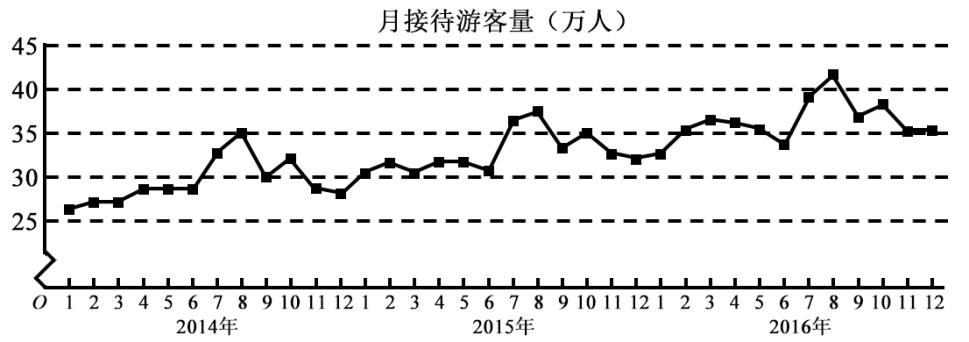
\includegraphics[width=0.85\textwidth]{Image/iii-3.jpg}
\end{figure}\\[-1.5em]
根据该折线图,下列结论错误的是
\begin{tasks}(1)
	\task 月接待游客量逐月增加 
	\task 年接待游客量逐年增加
	\task 各年的月接待游客量高峰期大致在7,8月份 
	\task 各年1月至6月的月接待游客量相对7月至12月,波动性更小,变化比较平稳 
\end{tasks}

\item $(x+y)(2x-y)^5$ 的展开式中 $x^3y^3$ 的系数为 
\begin{tasks}(4)
	\task $-80$ \task $-40$ \task $40$ \task $80$ 
\end{tasks}
\item 已知双曲线 $C\colon\,\tfrac{x^2}{a^2}-\tfrac{y^2}{b^2}=1\,(a>0,b>0)$ 的一条渐近线方程为 $y=\tfrac{\sqrt{5}}{2}x$ ,且与椭圆\\
 $\tfrac{x^2}{12}+\tfrac{y^2}{3}=1$ 有公共焦点,则 $C$ 的方程为
\begin{tasks}(4)
	\task $\frac{x^2}{8}-\frac{y^2}{10}=1$ \task $\frac{x^2}{4}-\frac{y^2}{5}=1$ \task $\frac{x^2}{5}-\frac{y^2}{4}=1$ \task $\frac{x^2}{4}-\frac{y^2}{3}=1$ 
\end{tasks}
\item 设函数 $f(x)=\cos\big(x+\tfrac{\pi}{3}\big)$,则下列结论错误的是
\begin{tasks}(2)
\task $f(x)$ 的一个周期为 $-2\pi$ \task $y=f(x)$ 的图像关于直线 $x=\frac{8\pi}{3}$ 对称
\task $f(x+\pi)$ 的一个零点为 $x=\frac{\pi}{6}$ \task  $f(x)$在 $\Big(\frac{\pi}{2},\pi\Big)$ 单调递减 
\end{tasks}

\item 执行右面的程序框图,为使输出 $S$ 的值小于 $91$,则输入的正整数 $N$ 的最小值为
\begin{figure}[htbp]
	\centering
	\includegraphics{Image/iii-7.pdf}
\end{figure}
\begin{tasks}(4)
	\task 5 \task 4 \task 3 \task 2 
\end{tasks}

\item 已知圆柱的高为1,它的两个底面的圆周在直径为2的同一个球的球面上,则该圆柱的体积为
\begin{tasks}(4)
	\task $\pi$ \task $\frac{3\pi}{4}$ \task $\frac{\pi}{2}$ \task 0 
\end{tasks}
\item 等差数列的首项为1,公差不为0. 若 $a_2$,$a_3$,$a_6$ 成等比数列,则前 6 项的和为
\begin{tasks}(4)
	\task $-24$ \task $-3$ \task 3 \task 8 
\end{tasks}
\item 已知椭圆 $C\colon\,\tfrac{x^2}{a^2}+\tfrac{y^2}{b^2}=1\,(a>b>0)$,的左、右顶点分别为 $A_1$,$A_2$,且以线段 $A_1A_2$ 为直径的圆与直线 $bx-ay+2ab=0$ 相切,则 $C$ 的离心率为
\begin{tasks}(4)
	\task $\frac{\sqrt{6}}{3}$ \task $\frac{\sqrt{3}}{3}$ \task $\frac{\sqrt{2}}{3}$ \task $\frac{1}{3}$ 
\end{tasks}
\item 已知函数 $f(x)=x^2-2x+a(e^{x-1}+e^{-x+1})$ 有唯一零点,则 $a=$
\begin{tasks}(4)
	\task $-\frac{1}{2}$ \task $\frac{1}{3}$ \task $\frac{1}{2}$ \task 1 
\end{tasks}
\item 在矩形 $ABCD$ 中,$AB=1$,$AD=2$,动点 $P$ 在以点 $C$ 为圆心且与 $BD$ 相切的圆上.\\
若 $\overrightarrow{\bfit{AP}}=\lambda\overrightarrow{\bfit{AB} }+\mu\overrightarrow{\bfit{AD}}$,则 $\lambda+\mu$ 的最大值为
\begin{tasks}(4)
	\task 3 \task $2\sqrt{2}$ \task $\sqrt{5}$ \task 2 
\end{tasks}
\end{enumerate}

\section{填空题:本题共4小题,每小题5分,共20分。}
\begin{enumerate}[itemsep=-0.3em,topsep=0pt,resume]%\setcounter{enumi}{12}
\item  若 $x$,$y$ 满足约束条件 $\left\{\begin{array}{@{}l}
x-y\geqslant0,\\x+y-2\leqslant0,\\y\geqslant0,
\end{array}\right.$
,则 $z=3x-4y$ 的最小值为 \blank{-1}.

\item 设等比数列 $\{a_n\}$ 满足 $a_1+a_2=–1$, $a_1–a_3=–3$,则 $a_4=$ \blank{-8}.

\item 设函数 $\biggl\lbrace\begin{array}{@{}ll}
x+1,&x\leqslant1\\2^x,&x>0
\end{array}$ 则满足的 $f(x)+f\big(x-\tfrac{1}{2}\big)>1$ 的 $x$ 取值范围是\blank{$(-1/4,+\infty)$}.
\item $a$,$b$ 为空间中两条互相垂直的直线,等腰直角三角形 $ABC$ 的直角边 $AC$ 所在直线与 $a$,$b$都垂直,斜边 $AB$ 以直线 $AC$ 为旋转轴旋转,有下列结论:
\begin{enumerate}[align=left,labelsep=-0.6em,leftmargin=1.2em,noitemsep,topsep=0pt]
	\item[\ding{172}] 当直线 $AB$ 与 $a$ 成 $60\,^{\circ}$ 角时, $AB$ 与 $b$ 成 $30\,^{\circ}$ 角;
	\item[\ding{173}] 当直线 $AB$ 与 $a$ 成 $60\,^{\circ}$ 角时, $AB$ 与 $b$ 成 $60\,^{\circ}$ 角;
	\item[\ding{174}] 直线 $AB$ 与 $a$ 所称角的最小值为 $45\,^{\circ}$ ;
	\item[\ding{175}] 直线 $AB$ 与 $a$ 所称角的最小值为 $60\,^{\circ}$ ;
\end{enumerate}
其中正确的是\blank{\ding{173}\ding{174}}.(填写所有正确结论的编号)
\end{enumerate}

\section{解答题:共70分。解答应写出文字说明、证明过程或演算步骤。第 $17\sim21$题为必考题,每个试题考生都必须作答。第22、23题为选考题,考生根据要求作答。}
\subsection{必考题:60分。}

\begin{enumerate}[itemsep=-0.3em,topsep=0pt,resume]%\setcounter{enumi}{17}
\item (12 分)\\
$\triangle$ $ABC$ 的内角 $A$,$B$,$C$ 的对边分别为 $a$,$b$,$c$,已知 $\sin A+\sqrt{3}\cos A=0$,$a=2\sqrt{7}$,$b=2$.
    \begin{enumerate}[itemsep=-0.3em,label={(\arabic*)},topsep=0pt,labelsep=.5em,leftmargin=1.7em]
	\item 求 $c$;
	\item 设 $D$ 为 $BC$ 边上一点,且 $AD\,\bot \,AC$,求 $\triangle$ $ABD$ 的面积.
    \end{enumerate}
\item (12 分)\\
某超市计划按月订购一种酸奶,每天进货量相同,进货成本每瓶4元,售价每瓶6元,未售出的酸奶降价处理,以每瓶2元的价格当天全部处学科网理完.根据往年销售经验,每天需求量与当天最高气温(单位:$\,^{\circ}\mathrm{C}$)有关.如果最高气温不低于25,需求量为500瓶;如果最高气温位于区间 $[25,30)$ ,需求量为300瓶;如果最高气温低于20,需求量为200瓶.为了确定六月份的订购计划,统计了前三年六月份各天的最高气温数据,得下面的频数分布表:\\[-2em]
\begin{table}[htbp]
\centering
\begin{tabular}{|c|c|c|c|c|c|c|c|}\hline
最高气温 & $[10,15)$& $[15,20)$ & $[20,25)$ & $[25,30)$ & $[30,35)$ & $[35,40)$\\\hline
天数     & 2        & 16       &36        &25        &7         &4         \\\hline
\end{tabular}
\end{table}\\[-1em]
以最高气温位于各区间的频率代替最高气温位于该区间的概率。
    \begin{enumerate}[itemsep=-0.3em,label={(\arabic*)},topsep=0pt,labelsep=.5em,leftmargin=1.7em]
	\item 求六月份这种酸奶一天的需求量 $X$(单位:瓶)的分布列;
	\item 设六月份一天销售这种酸奶的利润为 $Y$(单位:元),当六月份这种酸奶一天的进货量 $n$(单位:瓶)为多少时,$Y$ 的数学期望达到最大值?
    \end{enumerate}%\newpage
\item (12 分)\\[0.5em] \begin{minipage}[h][20ex][t]{.55\textwidth}
如图,四面体 $ABCD$ 中,$\triangle ABC$是正三角形,$\triangle ACD$是直角三角形,$\angle ABD=\angle CBD$,$AB=BD$.
\begin{enumerate}[itemsep=-0.3em,label={(\arabic*)},topsep=0pt,labelsep=.5em,leftmargin=1.7em]
	\item 证明:平面 $ACD\bot $ 平面 $ABC$;
	\item 过 $AC$ 的平面交 $BD$ 于点 $E$,若平面 $AEC$ 把四面体 $ABCD$ 分成体积相等的两部分,求二面角\\ $D-AE-C$的余弦值.
\end{enumerate}\end{minipage}
\begin{minipage}[h][20ex][t]{.45\textwidth}
	\includegraphics[width=6.5cm]{Image/iii-19.pdf}
\end{minipage}\vspace{3em}

\item (12 分)\\
已知抛物线 $C\colon\, y^2=2x$,过点 $(2,0)$ 的直线 $l$ 交 $C$ 与 $A$, $B$ 两点,圆 $M$ 是以线段 $AB$ 为直径的圆.
\begin{enumerate}[itemsep=-0.3em,label={(\arabic*)},topsep=0pt,labelsep=.5em,leftmargin=1.7em]
	\item 证明:坐标原点 $O$ 在圆 $M$ 上;
	\item 设圆 $M$ 过点 $P(4,-2)$,求直线 $l$ 与圆 $M$ 的方程.
\end{enumerate}

\item (12 分)\\
已知函数 $f(x)=x-1-a\ln x$.
\begin{enumerate}[itemsep=-0.3em,label={(\arabic*)},topsep=0pt,labelsep=.5em,leftmargin=1.7em]
	\item 若 $f(x)\geqslant0$,求 $a$ 的值;
	\item 设 $m$ 为整数,且对于任意正整数 $n$, $\left(1+\tfrac{1}{2}\right)\left(1+\tfrac{1}{2^2}\right)\cdots\left(1+\tfrac{1}{2^n}\right)<m$,求 $m$最小值.
\end{enumerate}
\end{enumerate}

\subsection{选考题:共10分。请考生在第22、23题中任选一题作答,如果多做,则按所做的第一题计分。}
\begin{enumerate}[resume]%\setcounter{enumi}{22}
\item \,[选修4―4:坐标系与参数方程]\, (10 分)\\
在直角坐标系 $xOy$ 中,直线 $l_1$ 的参数方程为 $\biggl\{\begin{array}{@{}l}
x=2+t,\\y=kt,
\end{array}$\, ($t$为参数),直线 $l_2$ 的参数方程为 $\Biggl\{\begin{array}{@{}l}
x=-2+m,\\[0.5mm]y=\frac{m}{k},
\end{array}$ ($m$ 为参数)
.设 $l_1$ 与$l_2$ 的交点为 $P$,当 $k$ 变化时,$P$ 的轨迹为曲线 $C$.
\begin{enumerate}[itemsep=-0.3em,label={(\arabic*)},topsep=0pt,labelsep=.5em,leftmargin=1.7em]
	\item 写出 $C$ 的普通方程;
	\item 以坐标原点为极点,$x$ 轴正半轴为极轴建立极坐标系,设 $l_3\colon\,\rho(\cos\theta+\sin\theta)-\sqrt{2}=0$,\\
	$M$ 为 $l_3$ 与 $C$ 的交点,求 $M$ 的极径.
\end{enumerate}
\item \,[选修4—5:不等式选讲]\, (10 分)\\
已知函数 $f(x)=|x+1|-|x-2|$.
\begin{enumerate}[itemsep=-0.3em,label={(\arabic*)},topsep=0pt,labelsep=.5em,leftmargin=1.7em]
	\item 求不等式 $f(x)\geqslant1$ 的解集;
	\item 若不等式$f(x)\geqslant x^2-x+m$ 的解集非空,求 $m$ 的取值范围.
\end{enumerate}
\end{enumerate}
 



%%%%%%%%%%%%%%%%%%%%%%%%%%%%%%%%%%%%%%%%%%%%%%%%%%%%%%%%%%%%%%%%%%%%%%%%%%
%---------------------------------结束------------------------------------
%%%%%%%%%%%%%%%%%%%%%%%%%%%%%%%%%%%%%%%%%%%%%%%%%%%%%%%%%%%%%%%%%%%%%%%%%%
\clearpage

\end{document}

%合并文档一面双页
% \documentclass{article}
% \usepackage{pdfpages}
% \usepackage[paperwidth=39.5cm,paperheight=27.2cm]{geometry}
% \begin{document}
% \includepdf[pages=1-6,nup=2x1]{dibajiefeishujuesaijuanzi.pdf}
% \end{document}
% doublepages
